%%%%%%%%%%%%%%%%%%%%%%%%%%%%%%%%%%%%%%%%%%%%%%%%%%%%%%%%%%%%%%%%%%%%%%%%%%%%%%%%%%%%%%%%%%
% Ceci est le fichier principal du template template à utiliser pour les rapports du     %
% projet 2 (TAD) d'INFO0947.                                                             %
%                                                                                        %
% Vous devez décommenter et compléter les commandes introduites plus bas (intitule, ...) %
% avant de pouvoir compiler le fichier LaTeX.  Pensez à configurer votre Makefile en     %
% conséquence.                                                                           %
%                                                                                        %
% Le contenu et la structure du rapport sont imposés.  Vous devez compléter les          %
% différents fichiers .tex inclus dans ce fichier avec votre production.                 %
%%%%%%%%%%%%%%%%%%%%%%%%%%%%%%%%%%%%%%%%%%%%%%%%%%%%%%%%%%%%%%%%%%%%%%%%%%%%%%%%%%%%%%%%%%

% !TEX root = ./main.tex
% !TEX engine = latexmk -pdf
% !TEX buildOnSave = true
\documentclass[a4paper, 11pt, oneside]{article}

\usepackage[utf8]{inputenc}
\usepackage[T1]{fontenc}
\usepackage[french]{babel}
\usepackage{array}
\usepackage{shortvrb}
\usepackage{listings}
\usepackage[fleqn]{amsmath}
\usepackage{amsfonts}
\usepackage{fullpage}
\usepackage{enumerate}
\usepackage{graphicx}             % import, scale, and rotate graphics
\usepackage{subfigure}            % group figures
\usepackage{alltt}
\usepackage{url}
\usepackage{indentfirst}
\usepackage{eurosym}
\usepackage{listings}
\usepackage{color}
\usepackage[table,xcdraw,dvipsnames]{xcolor}
\usepackage{multirow}

\definecolor{mygray}{rgb}{0.5,0.5,0.5}
\newcommand{\coms}[1]{\textcolor{MidnightBlue}{#1}}

\lstset{
    language=C, % Utilisation du langage C
    commentstyle={\color{MidnightBlue}}, % Couleur des commentaires
    frame=single, % Entoure le code d'un joli cadre
    rulecolor=\color{black}, % Couleur de la ligne qui forme le cadre
    stringstyle=\color{RawSienna}, % Couleur des chaines de caractères
    numbers=left, % Ajoute une numérotation des lignes à gauche
    numbersep=5pt, % Distance entre les numérots de lignes et le code
    numberstyle=\tiny\color{mygray}, % Couleur des numéros de lignes
    basicstyle=\tt\footnotesize,
    tabsize=3, % Largeur des tabulations par défaut
    keywordstyle=\tt\bf\footnotesize\color{Sepia}, % Style des mots-clés
    extendedchars=true,
    captionpos=b, % sets the caption-position to bottom
    texcl=true, % Commentaires sur une ligne interprétés en Latex
    showstringspaces=false, % Ne montre pas les espace dans les chaines de caractères
    escapeinside={(>}{<)}, % Permet de mettre du latex entre des <( et )>.
    inputencoding=utf8,
    literate=
  {á}{{\'a}}1 {é}{{\'e}}1 {í}{{\'i}}1 {ó}{{\'o}}1 {ú}{{\'u}}1
  {Á}{{\'A}}1 {É}{{\'E}}1 {Í}{{\'I}}1 {Ó}{{\'O}}1 {Ú}{{\'U}}1
  {à}{{\`a}}1 {è}{{\`e}}1 {ì}{{\`i}}1 {ò}{{\`o}}1 {ù}{{\`u}}1
  {À}{{\`A}}1 {È}{{\`E}}1 {Ì}{{\`I}}1 {Ò}{{\`O}}1 {Ù}{{\`U}}1
  {ä}{{\"a}}1 {ë}{{\"e}}1 {ï}{{\"i}}1 {ö}{{\"o}}1 {ü}{{\"u}}1
  {Ä}{{\"A}}1 {Ë}{{\"E}}1 {Ï}{{\"I}}1 {Ö}{{\"O}}1 {Ü}{{\"U}}1
  {â}{{\^a}}1 {ê}{{\^e}}1 {î}{{\^i}}1 {ô}{{\^o}}1 {û}{{\^u}}1
  {Â}{{\^A}}1 {Ê}{{\^E}}1 {Î}{{\^I}}1 {Ô}{{\^O}}1 {Û}{{\^U}}1
  {œ}{{\oe}}1 {Œ}{{\OE}}1 {æ}{{\ae}}1 {Æ}{{\AE}}1 {ß}{{\ss}}1
  {ű}{{\H{u}}}1 {Ű}{{\H{U}}}1 {ő}{{\H{o}}}1 {Ő}{{\H{O}}}1
  {ç}{{\c c}}1 {Ç}{{\c C}}1 {ø}{{\o}}1 {å}{{\r a}}1 {Å}{{\r A}}1
  {€}{{\euro}}1 {£}{{\pounds}}1 {«}{{\guillemotleft}}1
  {»}{{\guillemotright}}1 {ñ}{{\~n}}1 {Ñ}{{\~N}}1 {¿}{{?`}}1
}
\newcommand{\tablemat}{~}

%%%%%%%%%%%%%%%%% TITRE %%%%%%%%%%%%%%%%
% Complétez et décommentez les définitions de macros suivantes :
\newcommand{\intitule}{Le titre du travail}
 \newcommand{\GrNbr}{1742}
 \newcommand{\PrenomUN}{Galileo}
 \newcommand{\NomUN}{Galilei}
 \newcommand{\PrenomDEUX}{Octave}
 \newcommand{\NomDEUX}{Urbain}

\renewcommand{\tablemat}{\tableofcontents}

%%%%%%%% ZONE PROTÉGÉE : MODIFIEZ UNE DES DIX PROCHAINES %%%%%%%%
%%%%%%%%            LIGNES POUR PERDRE 2 PTS.            %%%%%%%%
\title{INFO0947: \intitule}
\author{Groupe \GrNbr : \PrenomUN~\textsc{\NomUN}, \PrenomDEUX~\textsc{\NomDEUX}}
\date{}
\begin{document}

\maketitle
\newpage
\tablemat
\newpage

%%%%%%%%%%%%%%%% RAPPORT %%%%%%%%%%%%%%%

% Inclusion des différentes sections

\section{Introduction}\label{introduction}

Ce projet consistait à développer une implémentation du jeu "Five or More", 
où le joueur doit déplacer des boules de différentes couleurs sur une grille en créant des 
alignements d'au moins cinq boules de même couleur, générant ainsi du score. 
Notre travail a porté sur la conception d'une interface graphique 
utilisant la bibliothèque GTK2+, ainsi que sur l'implémentation de la logique 
de jeu en langage C avec divers algorithmes.

% !TEX root = ./main.tex
%%%%%%%%%%%%%%%%%%%%%%%%%%%%%%%%%%%%%%%%%%%%%%%%%%%%%%%%%%%%%%%%%%%%%%%%%%%%%%%%%%%%%%%%%%
% Dans cette section, spécifiez formellement vos TADs (syntaxe et sémantique)            %
% 1 sous-section/TAD                                                                     %
% N'oubliez pas de justifier la complétude de vos TADs                                   %
%%%%%%%%%%%%%%%%%%%%%%%%%%%%%%%%%%%%%%%%%%%%%%%%%%%%%%%%%%%%%%%%%%%%%%%%%%%%%%%%%%%%%%%%%%
\section{Spécifications Abstraites}\label{tad}
%%%%%%%%%%%%%%%%%%%%%%%%%%%%%%%%%%%
À titre d'exemple, voici les spécifications abstraites pour le TAD \texttt{Vector} telles que vues dans le cours théorique (Chapitre 5).  À adapter en fonction de vos besoins pour le projet.

\subsection{TAD Vector}
%%%%%%%%%%%%%%%%%%%%%%%%
\subsubsection{Syntaxe}
%%%%%%%%%%%%%%%%%%%%%%%
\begin{description}
  \item[Type:]
    \begin{description}
      \item Vector
    \end{description}
  \item[Utilise:]
    \begin{description}
      \item Integer
      \item Element
    \end{description}
  \item[Opérations:]
    \begin{description}
      \item create: Integer $\to$ Vector
      \item set: Vector $\times$ Integer $\times$ Element $\to$ Vector
      \item get: Vector $\times$ Integer $\to$ Element
      \item size: Vector $\to$ Integer
    \end{description}
\end{description}

\subsubsection{Sémantique}
%%%%%%%%%%%%%%%%%%%%%%%%%%
\begin{description}
  \item[Préconditions:]
    \begin{description}
      \item $\forall i \in$ Integer, $\forall e \in$ Element, $\forall v\in$ Vector
      \item $\forall i \geq 0$, create(i)
      \item $\forall i,  0 \leq i <$ size(v), get(v, i)
      \item $\forall i, 0 \leq i <$ size(v), set(v, i, e)
    \end{description}
  \item[Axiomes:]
    \begin{description}
      \item $\forall e \in$ Element, $\forall v \in$ Vector, $\forall i, j \in$ Integer
      \item size(create(i)) = i
      \item size(set(v, i, e)) = size(v)
      \item get(set(v, i, e), j) =
      $\begin{cases}
        e         & \textrm{If}~i=j\\
        \textrm{get}(v, j) & \textrm{Otherwise}
      \end{cases}$
    \end{description}
\end{description}

\begin{table}[!htbp]
  \begin{center}
    \begin{tabular}{ll|cc}
      & & \multicolumn{2}{c}{Opérations Internes}\\
                                    &               & create($\cdot$) & set($\cdot$)\\
      \multirow{2}{*}{Observateurs} & get($\cdot$)  & $\emptyset$     & \checkmark\\
                                    & size($\cdot$) & \checkmark      & \checkmark\\
    \end{tabular}
  \end{center}
\end{table}



\section{Structures de données}\label{structures}

\subsection{Structures principales}

Nous avons conçu plusieurs structures de données opaques pour encapsuler les éléments du jeu. Voici leurs définitions complètes:

\begin{lstlisting}[language=C, caption=Structure Plateau\_t]
/**
 * @struct Plateau_t
 * @brief Structure principale representant le plateau de jeu
 */
typedef struct Plateau_t {
    int largeur;              // Nombre de colonnes
    int hauteur;              // Nombre de lignes
    int nb_types_symboles;    // Nombre de couleurs differentes
    int symboles_par_tour;    // Nombre de boules par tour
    int nb_cases_remplies;    // Nombre de cases occupees
    Case **cases;             // Tableau 2D des cases du plateau
    int difficulte;           // Niveau de difficulte
    Score score;              // Score actuel
    int nb_suivantes;         // Nombre de boules suivantes
    Couleur boules_suivantes[MAX_SUIVANTS];// Tableau des couleurs des boules suivantes
    GtkWidget **boutons_suivants;  // Boutons representant les boules suivantes
} Plateau;
\end{lstlisting}

\begin{lstlisting}[language=C, caption=Structure Case\_t]
/**
 * @struct Case_t
 * @brief Structure representant une case du plateau de jeu
 */
typedef struct Case_t {
    bool occupe;       // Indique si la case contient une boule
    Couleur col;       // Couleur de la boule (si presente)
    GtkWidget *image;  // Bouton GTK representant la case
} Case;
\end{lstlisting}

\begin{lstlisting}[language=C, caption=Structure Score\_t]
/**
 * @struct Score_t
 * @brief Structure representant un score dans le jeu
 */
typedef struct Score_t {
    char nom[MAX_NOM + 1];  // Nom du joueur
    int valeur;             // Valeur du score
} Score;
\end{lstlisting}

\begin{lstlisting}[language=C, caption=Structure Boule\_t]
/**
 * @struct Boule_t
 * @brief Structure representant une boule
 */
typedef struct Boule_t {
    Couleur couleur;    // Couleur de la boule
    GtkWidget *image;   // Image associee a la boule
} Boule;
\end{lstlisting}

\subsection{Structures auxiliaires}

En plus des structures principales, nous utilisons des structures auxiliaires pour faciliter certaines opérations:

\begin{lstlisting}[language=C, caption=Structure MiseAJour]
/**
 * @brief Structure utilisee pour la mise a jour des cases 
 * et la recherche de boutons
 */
typedef struct {
    int ligne_actuelle;      // Coordonnee ligne de la case recherchee
    int colonne_actuelle;    // Coordonnee colonne de la case recherchee
    Plateau *plateau;        // Plateau de jeu concerne
    GtkWidget *est_bouton;   // Bouton trouve
    GtkWidget *bouton_trouve;// Bouton trouve (alternative)
} MiseAJour;
\end{lstlisting}

\begin{lstlisting}[language=C, caption=Structure Data]
/**
 * @brief Structure utilisee pour les recherches de widgets dans l'interface
 */
typedef struct {
    GtkWidget *est_widget;   // Widget trouve
    gboolean est_trouve;     // Indique si un widget a ete trouve
} Data;
\end{lstlisting}

\begin{lstlisting}[language=C, caption=Structure InfosCallback]
   /**
    * @brief Structure utilisee pour stocker des informations dans les callbacks
    */
   typedef struct {
       int ligne_actuelle;      // Coordonnee ligne de la case courante
       int colonne_actuelle;    // Coordonnee colonne de la case courante
       Plateau *plateau;        // Plateau de jeu concerne
   } InfosCallback;
   \end{lstlisting}

% !TEX root = ./main.tex
%%%%%%%%%%%%%%%%%%%%%%%%%%%%%%%%%%%%%%%%%%%%%%%%%%%%%%%%%%%%%%%%%%%%%%%%%%%%%%%%%%%%%%%%%%
% Dans cette section, spécifiez formellement chacun des sous-problèmes.                  %
%%%%%%%%%%%%%%%%%%%%%%%%%%%%%%%%%%%%%%%%%%%%%%%%%%%%%%%%%%%%%%%%%%%%%%%%%%%%%%%%%%%%%%%%%%
\section{Specifications}\label{specifications}
%%%%%%%%%%%%%%%%%%%%%%%%

%  \item \textbf{SP1} : \'Enumération des tailles possbiles de préfixe-suffixe.
%\item \textbf{SP2} : Comparer les valeurs de préfixe et de suffixe.

\subsection{Sous-problème 1}
Nous voulons écrire une boucle dans laquelle $k$ balaye toutes les valeurs
possibles pour le préfixe-suffixe. Pour ceci définissons la fonction:
\begin{itemize}
   \item \textbf{Input:}
      \begin{itemize}
         \item $N$, la taille du tableau
      \end{itemize}
   \item \textbf{Output:}
      \begin{itemize}
         \item $k$, la taille du préfixe-suffixe
      \end{itemize}
   \item \textbf{Caractérisation de l'input:}
      \begin{itemize}
         \item $N$ est un entier non signé tel que $N \geq 0$
         \item \textbf{unsigned int} N
      \end{itemize}
\end{itemize}

\vspace{0.4cm}
Il nous faut donc écrire une boucle while qui va balayer toutes les valeurs 
possibles de $k$ de $N-1$ à 0.
\begin{itemize}
   \item \textbf{Déclaration du compteur:}
      \begin{itemize}
         \item \textbf{unsigned int} $k = N-1$
      \end{itemize}
   \item \textbf{Nombres de tours dans la boucle:}
      \begin{itemize}
         \item $N-1$
      \end{itemize}
   \item \textbf{Gardien de boucle:}
      \begin{itemize}
         \item $k > 0$
      \end{itemize}
   \item \textbf{Corps de Boucle:}
   \begin{itemize}
      \item \textbf{Comparer les valeurs de préfixe et de suffixe:}
      \begin{itemize}
         \item SP2
      \end{itemize}
      \item Décrémenter k
   \end{itemize}
\end{itemize}

\begin{lstlisting}[language=C, caption=SP1]
unsigned int k = N - 1;
while (k > 0) {
   // SP2
   k--;
}
\end{lstlisting}

\subsection{Sous-problème 2}
Nous voulons écrire une boucle dans laquelle on compare les valeurs de préfixe
et de suffixe. Pour ceci définissons la fonction:
\begin{itemize}
   \item \textbf{Input:}
      \begin{itemize}
         \item $T$, le tableau d'entiers
         \item $N$, la taille du tableau
         \item $k$, la taille du préfixe-suffixe
         \item $i$, le compteur de la boucle
      \end{itemize}
   \item \textbf{Output:}
      \begin{itemize}
         \item $k$, la taille du préfixe-suffixe
      \end{itemize}
   \item \textbf{Caractérisation des inputs:}
      \begin{itemize}
         \item $N$ est un entier non signé tel que $N \geq 0$
         \item \textbf{unsigned int} $N$
         \item $k$ est un entier non signé tel que $0 \leq k < N$
         \item \textbf{unsigned int} $k = N - 1$
         \item $i$ est un entier non signé tel que $0 \leq i < k$
         \item \textbf{unsigned int} $i = 0$
         \item $T$ est un tableau d'entiers tel que $T[0, N-1]$
         \item \textbf{int} $T[N]$
      \end{itemize}
\end{itemize}
%
%
%
%
%
%%%%%%%%%%%%%%%%%%%%%%%%%%%% A CONTINUER %%%%%%%%%%%%%%%%%%%%%%%%%%%%%%%%

\vspace{0.4cm}
Il nous faut donc écrire une boucle while qui va balayer toutes les valeurs
possibles de $i$ de 0 à k-1 et trouver des correspondances entre les
valeurs de préfixe $i$ et de suffixe $N-k+i$.
\begin{itemize}
   \item \textbf{Déclaration du compteur:}
      \begin{itemize}
         \item \textbf{unsigned int} $i = 0$
      \end{itemize}
   \item \textbf{Nombres de tours dans la boucle:}
      \begin{itemize}
         \item $k$
      \end{itemize}
   \item \textbf{Gardien de boucle:}
   \item \textbf{Condition de sortie:}
      \begin{itemize}
         \item $i < k $\space$ \&\& $\space$ T[i] == T[N - k +i]$
      \end{itemize}
   \item \textbf{Corps de Boucle:}
   \begin{itemize}
      \item \textbf{Vérifier si $i$ et $k$ sont égaux:}
      \begin{itemize}
      \item if (i == k)
      \end{itemize}
      \item Incrémenter i
   \end{itemize}
\end{itemize}

\vspace{0.4cm}
\begin{lstlisting}[language=C, caption=SP2]
unsigned int i = 0;
while(i < k && T[i] == T[N - k +i]){
   i++;
   }
   if (i == k){
      return k;
   }
   else{
      i = 0;
}
\end{lstlisting}

% !TEX root = ./main.tex
%%%%%%%%%%%%%%%%%%%%%%%%%%%%%%%%%%%%%%%%%%%%%%%%%%%%%%%%%%%%%%%%%%%%%%%%%%%%%%%%%%%%%%%%%%
% Dans cette section, indiquez et décrivez tous les Invariants nécessaires.              %
%                                                                                        %
% Pour chaque SP nécessitant un Invariant (une sous-section/SP):                         %
% - Donnez l'Invariant Graphique                                                         %
% - Donnez l'Invariant Formel correspondant à l'Invariant Graphique                      %
% Pensez à utiliser les notations définies précédemment.                                 %
%%%%%%%%%%%%%%%%%%%%%%%%%%%%%%%%%%%%%%%%%%%%%%%%%%%%%%%%%%%%%%%%%%%%%%%%%%%%%%%%%%%%%%%%%%
\section{Invariants}\label{invariants}
%%%%%%%%%%%%%%%%%%%%
\subsection{Explications}
La raison d'être de cette section est de définir les invariants nécessaires à la
construction du programme. Les invariants sont des propriétés qui doivent être
vérifiées à chaque étape de l'exécution du programme. Ils permettent de garantir
que le programme fonctionne correctement et produit les résultats attendus. Il y
a une règle qui est que chaque boucle nécessite un invriant. Nous aurons donc 2
invariants graphiques et 2 invariants formels

Nous allons donc définir les invariants graphiques. Le premier aura pour objectif
de définir la boucle de décrementation de $k$ et le seconde couvrira la boucle
qui compare les valeurs du tableau entre $T[i]$ et $T[N-k+i]$.

\subsection{SP1}
\subsubsection{Invariant Graphique}
Pour le premier invariant, nous allons définir la boucle de décrementation de $k
$. La valeur de $k$ est initialisée à $N - 1$ et elle est décrémentée jusqu'à ce
qu'elle atteigne 0. Attention, elle atteint zéro uniquement si lors du SP2 nous 
n'avons trouvé aucune correspondance dans le tableau.
\begin{figure}[h]
   \centering
   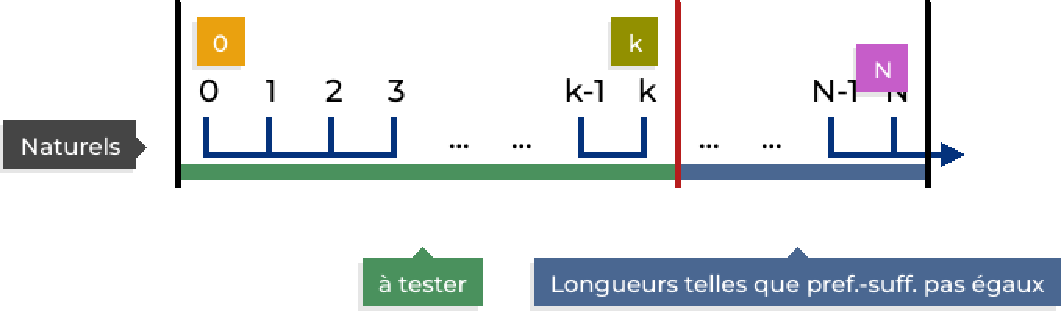
\includegraphics[width=0.5\textwidth]{sp1.pdf}
   \caption{Invariant graphique 1}
   \label{fig:invariant1}
\end{figure}

Le critère d'arrêt de la boucle est $k ==0$. Donc, le gardien de boucle sera
$k > 0$.

\subsubsection{Invariant Formel}

\begin{center}
   \fbox{
      \begin{minipage}{0.5\textwidth}
      \begin{center}
      $N = N_0$ \\
      $\wedge$ \\
      $ 0 \leq k \leq N - 1$ \\
      $\wedge$ \\
      k != max\_prefixe\_suffixe(*T, i ,N) \\
      \end{center}
      \end{minipage}
   }
\end{center}

\subsection{SP2}
\subsubsection{Invariant Graphique}
Pour le second invariant, nous allons définir la boucle de comparaison entre les
valeurs du tableau entre $T[i]$ et $T[N-k+i]$. La valeur de $i$ est initialisée 
à 0 et elle est incrémentée jusqu'à ce qu'elle atteigne $k$.

\begin{figure}[h]
   \centering
   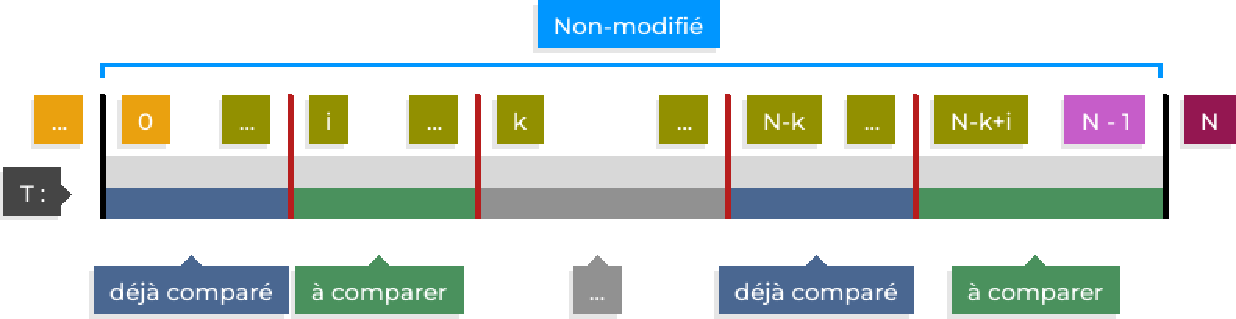
\includegraphics[width=0.5\textwidth]{sp2.pdf}
   \caption{Invariant graphique 2}
   \label{fig:invariant2}
\end{figure}

Le critère d'arrêt de la boucle est $i == k$. Donc, le gardien de boucle sera
$i < k$.
\subsubsection{Invariant Formel}

\begin{center}
   \fbox{
      \begin{minipage}{0.5\textwidth}
      \begin{center}
      $N = N_0 \wedge T = T_0$ \\
      $\wedge$ \\
      $ 0 \leq i < k$ $< N$\\
      $\wedge$ \\
      $\forall i,k, 0 \leq i < k < N$, $est\_pre\_suff$ \\
      \end{center}
      \end{minipage}
   }
\end{center}

% !TEX root = ./main.tex
%%%%%%%%%%%%%%%%%%%%%%%%%%%%%%%%%%%%%%%%%%%%%%%%%%%%%%%%%%%%%%%%%%%%%%%%%%%%%%%%%%%%%%%%%%
% Justifiez, dans cette section, chacune de vos implémentations récursives à l'aide des  %
% 3 étapes vues au cours (cfr. Chap. 4)                                                  %
%%%%%%%%%%%%%%%%%%%%%%%%%%%%%%%%%%%%%%%%%%%%%%%%%%%%%%%%%%%%%%%%%%%%%%%%%%%%%%%%%%%%%%%%%%
\section{Implémentations Récursives}\label{recursivite}
%%%%%%%%%%%%%%%%%%%%%%%%%%%%%%%%%%%%%

Rappel de la signature de la fonction en C: 


Définition récursive:

nameF(arg1,..., argN) = $            
                \begin{cases}
                    ... & \text{if } ... \\
                    ... & \text{if } ... \\
                            ...          \\
                    ... & \text{otherwise}
                \end{cases} $




% !TEX root = ./main.tex
%%%%%%%%%%%%%%%%%%%%%%%%%%%%%%%%%%%%%%%%%%%%%%%%%%%%%%%%%%%%%%%%%%%%%%%%%%%%%%%%%%%%%%%%%%
% Dans cette section, vous devez étudier complètement la complexité de votre code.       %
% Soyez le plus formel (i.e., mathématique) possible.                                    %
%%%%%%%%%%%%%%%%%%%%%%%%%%%%%%%%%%%%%%%%%%%%%%%%%%%%%%%%%%%%%%%%%%%%%%%%%%%%%%%%%%%%%%%%%%
\section{Complexité}\label{complexite}
%%%%%%%%%%%%%%%%%%%%


% !TEX root = ./main.tex
%%%%%%%%%%%%%%%%%%%%%%%%%%%%%%%%%%%%%%%%%%%%%%%%%%%%%%%%%%%%%%%%%%%%%%%%%%%%%%%%%%%%%%%%%%
% Dans cette section, décrivez comment vous avez implémenté les différents tests         %
% unitaires                                                                              %
% Pensez à justifier vos choix.                                                          %
%%%%%%%%%%%%%%%%%%%%%%%%%%%%%%%%%%%%%%%%%%%%%%%%%%%%%%%%%%%%%%%%%%%%%%%%%%%%%%%%%%%%%%%%%%
\section{Tests Unitaires}\label{tests}
%%%%%%%%%%%%%%%%%%%%%%%%%


% !TEX root = ./main.tex
%%%%%%%%%%%%%%%%%%%%%%%%%%%%%%%%%%%%%%%%%%%%%%%%%%%%%%%%%%%%%%%%%%%%%%%%%%%%%%%%%%%%%%%%%%
% Rédigez ici la conclusion de votre rapport.                                            %
%%%%%%%%%%%%%%%%%%%%%%%%%%%%%%%%%%%%%%%%%%%%%%%%%%%%%%%%%%%%%%%%%%%%%%%%%%%%%%%%%%%%%%%%%%
\section{Conclusion}\label{conclusion}
%%%%%%%%%%%%%%%%%%%%%
Pour conclure, à travers notre rapport, nous avons établi une approche
constructive pour une fonction calculant le plus long
sous-tableau qui est à la fois préfixe et suffixe d'un tableau donné. 
Nous avons défini le problème, formalisé le problème, analysé, découpé en 
sous-problèmes et avons fait une approche constructive sur la base de nos invariants.

\vspace{0.4cm}
Nous avons également calculé la complexité de notre algorithme, qui est $O(n^2)$.
Notre code peut désormais être utilisé pour résoudre le problème de manière efficace et
fiable.

%%%%%%%%%%%%%%%%%%%% FIN DE LA ZONE PROTÉGÉE %%%%%%%%%%%%%%%%%%%%

\end{document}
